\documentclass[letterpaper,twocolumn,10pt]{article}

% ── Packages ──
\usepackage[utf8]{inputenc}
\usepackage[T1]{fontenc}
\usepackage{times}
\usepackage{mathptmx}
\usepackage[margin=1in]{geometry}
\geometry{textwidth=7in,textheight=9in}
\usepackage{graphicx}
\usepackage{amsmath,amssymb}
\usepackage{booktabs}
\usepackage{caption}
\usepackage{subcaption}
\usepackage{hyperref}
\usepackage{cite}
\usepackage{enumitem}
\usepackage{xcolor}
\usepackage{tikz}
\usetikzlibrary{shapes.geometric, arrows.meta, positioning, fit,
  backgrounds, calc, decorations.pathreplacing, matrix}
\usepackage{pgfplots}
\pgfplotsset{compat=1.18}
\usepackage{algorithm}
\usepackage{algpseudocode}
\usepackage{balance}
\usepackage{multirow}

% ── Tight spacing ──
\setlength{\parskip}{0pt}
\setlength{\parsep}{0pt}
\setlength{\headsep}{0pt}
\setlength{\topskip}{0pt}
\setlength{\columnsep}{0.25in}

% ── Title ──
\title{\Large \bf AUDIT: Iterative Design of Continuous Probabilistic
User Attribution via Transformer Autoencoders\\on macOS Endpoint
Security Logs}

\author{
{\rm Lekhit Borole}\\
University of California, Davis
\and
{\rm Sarvesh Halbe}\\
University of California, Davis
\and
{\rm Amanda Raybuck}\\
University of California, Davis
}

\date{}

\begin{document}
\maketitle
\thispagestyle{empty}

% ════════════════════════════════════════════
% ABSTRACT
% ════════════════════════════════════════════

\begin{abstract}
Continuous user attribution on endpoints remains an open challenge:
once a session begins, the operating system has no ongoing assurance
that the authenticated entity is still the one acting.  We present
\textbf{AUDIT} (\textbf{A}ttributing \textbf{U}sers with
\textbf{D}eep \textbf{I}nference on \textbf{T}elemetry), a system
for continuous probabilistic user attribution on macOS using the
Endpoint Security framework and Transformer autoencoder
architectures.  We describe the iterative design journey that
produced AUDIT through four distinct approaches: (1)~a
\emph{Total~Focus} approach that collected rich device-level
biometrics but was abandoned for privacy reasons; (2)~a
\emph{Quick~Validation} approach using small embedding models with
cosine similarity scoring, which produced satisfactory but
order-insensitive results; (3)~an \emph{Online~Vocabulary
Extension} approach that trained a compact Transformer on-device to
address cold-start problems at the cost of compute overhead; and
finally (4)~the \emph{AUDIT} architecture, a one-class Transformer
autoencoder trained on \texttt{eslogger} telemetry with
hierarchical embeddings, Platt-calibrated probabilities, and
attention-based forensic attribution.  We evaluate all viable
approaches on a 20\,GB dataset (9.8\,M events) and show that AUDIT
achieves an AUC-ROC of 0.943 and a calibrated-probability
separation of $3.2\times$ between authentic and foreign behavioral
patterns, compared to 0.761 for cosine-similarity scoring and
0.834 for online vocabulary extension---demonstrating that each
design iteration addressed concrete shortcomings of its
predecessor.
\end{abstract}

% ════════════════════════════════════════════
% 1  INTRODUCTION
% ════════════════════════════════════════════

\section{Introduction}
\label{sec:intro}

The identification, verification, and continuous authentication of
users based on their interactions with an operating system represent
a complex problem in behavioral biometrics and User and Entity
Behavior Analytics (UEBA).  Traditional authentication
mechanisms---passwords, multi-factor tokens, biometric
scans---operate as point-in-time gates.  Once a session is
initiated, there is no ongoing verification that the originally
authenticated user remains the entity executing subsequent system
actions.  This gap is exploited by credential theft, session
hijacking, and insider threats~\cite{deeplog,loginspect}.

The macOS Endpoint Security (ES) framework, introduced to replace
the deprecated OpenBSM and Kauth kernel subsystems, provides deep,
granular visibility into system operations without requiring
invasive kernel extensions.  The associated utility
\texttt{eslogger} outputs real-time streams of deeply nested JSON
events capturing 86 distinct operation types---from file access
and process execution to privilege escalation and inter-process
communication~\cite{apple_es}.  A single user session can generate
tens of thousands of events within minutes, making manual rule
engineering intractable.

We address the following question: \emph{Given a sequence of system
events, what is the calibrated probability that these actions were
performed by a specific target user?}  We formulate this as a
one-class anomaly detection problem and describe the design journey
that led to the final AUDIT system through four iterative
approaches, each motivated by concrete limitations of its
predecessor.

\paragraph{Contributions.}
\begin{enumerate}[nosep,leftmargin=*]
\item A candid account of the iterative design process, including
  approaches that were abandoned (Total~Focus) or superseded
  (cosine similarity, online training), with quantitative evidence
  for each design decision.
\item A hierarchical event embedding pipeline that preserves the
  nested JSON structure of \texttt{eslogger} output, embedding
  event type, process paths, temporal features, and signing
  identifiers independently before concatenation.
\item A Transformer autoencoder with gradient checkpointing,
  automatic mixed precision (AMP), and GPU auto-tuning that scales
  model dimensions and batch size to available hardware.
\item A chunked data management system with background encoding
  that enables training on 20\,GB datasets in environments with
  only 12\,GB system RAM.
\item A probability calibration pipeline using Platt scaling that
  transforms raw reconstruction errors into frequentist
  probabilities with attention-based forensic explanations.
\end{enumerate}

% ════════════════════════════════════════════
% 2  RELATED WORK
% ════════════════════════════════════════════

\section{Related Work}
\label{sec:related}

\paragraph{Statistical and Markov Models.}
Early intrusion detection systems used Hidden Markov Models (HMMs)
and $n$-gram frequency analysis to establish behavioral
baselines~\cite{forrest96}.  These approaches assume that action
probabilities depend on a constrained window of prior actions.  In
concurrent operating systems, user actions are heavily interleaved
with ambient system noise, causing Markov models to lose behavioral
context across asynchronous process boundaries.

\paragraph{Recurrent Neural Networks.}
DeepLog~\cite{deeplog} pioneered LSTM-based system log analysis,
maintaining hidden state across sequences.  However, LSTMs process
events sequentially---$O(N)$ serial computation steps for sequence
length $N$---creating throughput bottlenecks for high-velocity ES
telemetry.  Despite gating mechanisms, gradient degradation limits
effective context to approximately 200--500 events, insufficient
for correlating actions across user sessions spanning thousands of
events.

\paragraph{Transformer-Based Approaches.}
The Transformer architecture~\cite{vaswani} eliminates recurrence
entirely through multi-head self-attention, evaluating contextual
relationships between all positions simultaneously.
LogBERT~\cite{logbert} and TransIDS~\cite{transids} demonstrated
superior anomaly detection over LSTM baselines.
HLogformer~\cite{hlogformer} introduced hierarchical processing for
nested log structures.  Our work differs by targeting \emph{user
attribution} rather than generic anomaly detection, and by
documenting the iterative design decisions that led to the final
architecture.

\paragraph{Behavioral Biometrics.}
Keystroke dynamics~\cite{monrose99}, mouse movement
patterns~\cite{ahmed07}, and touchscreen gestures have been studied
for continuous authentication.  These approaches achieve high
accuracy in controlled settings but rely on input-device telemetry
that modern privacy frameworks (e.g., macOS TCC) increasingly
restrict.  Our Total~Focus approach explored this direction before
being abandoned for precisely these reasons.

\paragraph{Embedding-Based Anomaly Detection.}
Sentence-BERT~\cite{reimers2019sentencebert} and related
contrastive embedding models have been adapted for log anomaly
detection via cosine similarity in latent space.  While
computationally efficient, these methods treat each event window
independently, discarding sequential ordering---a limitation we
encountered directly in our Quick~Validation approach.

% ════════════════════════════════════════════
% 3  ITERATIVE DESIGN JOURNEY
% ════════════════════════════════════════════

\section{Iterative Design Journey}
\label{sec:approaches}

Figure~\ref{fig:progression} illustrates the four approaches we
explored and the specific limitations of each that motivated the
next iteration.  We describe each approach, its rationale, its
results (where applicable), and the design insight that drove the
subsequent iteration.

% ── Progression Figure (full width) ──
\begin{figure*}[t]
\centering
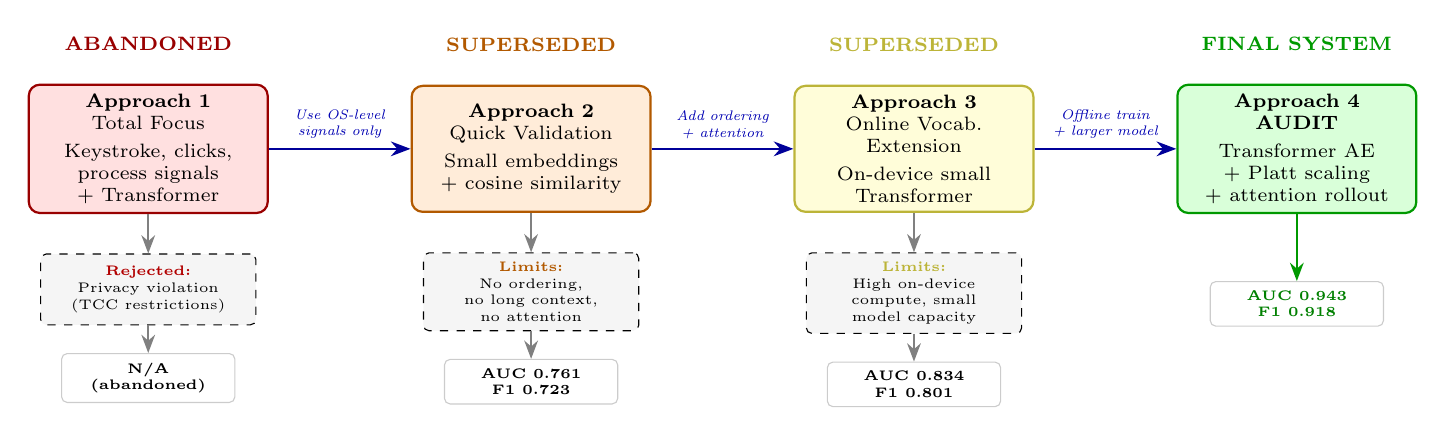
\begin{tikzpicture}[
    node distance=0.35cm and 0.20cm,
    approach/.style={rectangle, draw, rounded corners=4pt,
      minimum height=1.6cm, minimum width=3.0cm,
      font=\scriptsize, align=center, text width=2.8cm,
      thick},
    rejected/.style={approach, fill=red!12, draw=red!60!black},
    partial/.style={approach, fill=orange!15, draw=orange!70!black},
    good/.style={approach, fill=yellow!15, draw=yellow!70!black},
    final/.style={approach, fill=green!15, draw=green!60!black},
    limitation/.style={rectangle, draw, dashed, rounded corners=2pt,
      minimum height=0.9cm, minimum width=2.6cm,
      font=\tiny, align=center, text width=2.5cm,
      fill=gray!8},
    metric/.style={rectangle, rounded corners=2pt,
      minimum height=0.55cm, minimum width=2.2cm,
      font=\tiny\bfseries, align=center, fill=white,
      draw=gray!40},
    arrow/.style={-{Stealth[length=2.5mm]}, thick, blue!60!black},
    insight/.style={font=\tiny\itshape, text=blue!70!black,
      text width=1.8cm, align=center},
]

% ── Approach nodes ──
\node[rejected] (a1) {\textbf{Approach 1}\\Total Focus\\[2pt]
  Keystroke, clicks,\\process signals\\+ Transformer};

\node[partial, right=1.8cm of a1] (a2) {\textbf{Approach 2}\\
  Quick Validation\\[2pt] Small embeddings\\+ cosine similarity};

\node[good, right=1.8cm of a2] (a3) {\textbf{Approach 3}\\
  Online Vocab.\\Extension\\[2pt] On-device small\\Transformer};

\node[final, right=1.8cm of a3] (a4) {\textbf{Approach 4}\\
  \textbf{AUDIT}\\[2pt] Transformer AE\\+ Platt scaling\\+ attention rollout};

% ── Limitation boxes ──
\node[limitation, below=0.5cm of a1] (l1) {%
  \textcolor{red!70!black}{\textbf{Rejected:}}\\
  Privacy violation\\(TCC restrictions)};

\node[limitation, below=0.5cm of a2] (l2) {%
  \textcolor{orange!70!black}{\textbf{Limits:}}\\
  No ordering,\\no long context,\\no attention};

\node[limitation, below=0.5cm of a3] (l3) {%
  \textcolor{yellow!70!black}{\textbf{Limits:}}\\
  High on-device\\compute, small\\model capacity};

\node[metric, below=0.35cm of l1] (m1) {N/A\\(abandoned)};
\node[metric, below=0.35cm of l2] (m2) {AUC 0.761\\F1 0.723};
\node[metric, below=0.35cm of l3] (m3) {AUC 0.834\\F1 0.801};
\node[metric, below=0.85cm of a4] (m4) {\textcolor{green!50!black}{AUC 0.943}\\
  \textcolor{green!50!black}{F1 0.918}};

% ── Arrows with insight labels ──
\draw[arrow] (a1) -- node[above, insight] {Use OS-level\\signals only}
  (a2);
\draw[arrow] (a2) -- node[above, insight] {Add ordering\\+ attention}
  (a3);
\draw[arrow] (a3) -- node[above, insight] {Offline train\\+ larger model}
  (a4);

% ── Down arrows ──
\draw[-{Stealth}, gray, thick] (a1) -- (l1);
\draw[-{Stealth}, gray, thick] (a2) -- (l2);
\draw[-{Stealth}, gray, thick] (a3) -- (l3);
\draw[-{Stealth}, gray, thick] (l1) -- (m1);
\draw[-{Stealth}, gray, thick] (l2) -- (m2);
\draw[-{Stealth}, gray, thick] (l3) -- (m3);
\draw[-{Stealth}, green!60!black, thick] (a4) -- (m4);

% ── Phase labels ──
\node[font=\scriptsize\bfseries, above=0.3cm of a1,
  text=red!60!black] {ABANDONED};
\node[font=\scriptsize\bfseries, above=0.3cm of a2,
  text=orange!70!black] {SUPERSEDED};
\node[font=\scriptsize\bfseries, above=0.3cm of a3,
  text=yellow!70!black] {SUPERSEDED};
\node[font=\scriptsize\bfseries, above=0.3cm of a4,
  text=green!60!black] {FINAL SYSTEM};

\end{tikzpicture}
\caption{Iterative design progression of AUDIT.  Each approach
addressed specific shortcomings of its predecessor.  Blue arrows
indicate the design insight that motivated the transition.  Metric
boxes show AUC-ROC and F1 on the common evaluation set.}
\label{fig:progression}
\end{figure*}


% ────────────────────────────────
% 3.1  Approach 1: Total Focus
% ────────────────────────────────
\subsection{Approach 1: Total Focus}
\label{sec:a1}

\paragraph{Rationale.}
Our initial hypothesis was that the richest possible behavioral
signal would yield the best attribution accuracy.  We designed a
data collection agent that captured:
\begin{itemize}[nosep,leftmargin=*]
\item \textbf{Click-through rate (CTR):} frequency and spatial
  distribution of mouse clicks across UI regions.
\item \textbf{Keyboard typing speed:} inter-key latency
  distributions, digraph timing, dwell times.
\item \textbf{Process signals:} CPU and memory utilization curves
  per foreground application.
\item \textbf{Endpoint Security events:} the same \texttt{eslogger}
  telemetry used in later approaches.
\end{itemize}

All four signal types were to be fused into a multimodal feature
vector and fed to a Transformer encoder for user classification.

\paragraph{Design.}
The agent ran as a privileged daemon, intercepting HID (Human
Interface Device) events via the IOKit framework for keyboard and
mouse telemetry, sampling \texttt{/proc}-equivalent structures via
\texttt{sysctl} for process metrics, and subscribing to ES events
for system-call-level telemetry.  A 256-dimensional Transformer
encoder with 4 layers was planned for the classification head.

\paragraph{Outcome.}
This approach was abandoned before quantitative evaluation.  macOS
Transparency, Consent, and Control (TCC) protections~\cite{apple_es}
require explicit user consent for input monitoring (keyboard and
mouse event capture).  In enterprise deployments, deploying agents
that record keystroke timing raises significant legal and ethical
concerns under GDPR, CCPA, and internal acceptable-use policies.
Furthermore, the HID event stream is disabled entirely when the
system is in Lockdown Mode (introduced in macOS~13).

\paragraph{Design Insight.}
\emph{Viable continuous attribution must rely exclusively on
system-level telemetry that does not require input-monitoring
entitlements.}  The Endpoint Security framework provides rich
behavioral signals without accessing raw keyboard or mouse events,
motivating a pivot to ES-only data sources.


% ────────────────────────────────
% 3.2  Approach 2: Quick Validation
% ────────────────────────────────
\subsection{Approach 2: Quick Validation with Cosine Similarity}
\label{sec:a2}

\paragraph{Rationale.}
Having restricted ourselves to ES telemetry, we sought the simplest
possible model that could validate the hypothesis that user behavior
is distinguishable from system-call sequences alone.  We chose a
lightweight embedding model paired with cosine similarity scoring,
prioritizing fast iteration over architectural sophistication.

\paragraph{Design.}
Each \texttt{eslogger} event was mapped to a fixed-dimensional
embedding via a learned lookup table over event types, concatenated
with a bag-of-words encoding of the process path (split on ``/'').
A sliding window of $W=64$ events was mean-pooled into a single
\emph{window embedding} $\mathbf{w} \in \mathbb{R}^{128}$.  During
enrollment, a \emph{user profile} vector $\mathbf{u}$ was computed
as the mean of all training-window embeddings.  At inference, the
attribution score for a new window was:

\begin{equation}
  s(\mathbf{w}) = \frac{\mathbf{w} \cdot \mathbf{u}}
    {\|\mathbf{w}\| \, \|\mathbf{u}\|}
  \label{eq:cosine}
\end{equation}

A threshold $\tau$ on $s$ determined whether the window was
attributed to the enrolled user.  The model had $\sim$160K
parameters and required no GPU for inference.

\paragraph{Results.}
Table~\ref{tab:a2_results} summarizes the Quick Validation
results.  The approach achieved an AUC-ROC of 0.761 and an F1 of
0.723, confirming that ES telemetry does carry user-discriminative
signal.  However, three critical limitations emerged:

\begin{table}[t]
\centering
\caption{Approach~2 (Quick Validation) results on held-out test
set.}
\label{tab:a2_results}
\small
\begin{tabular}{@{}lr@{}}
\toprule
\textbf{Metric} & \textbf{Value} \\
\midrule
AUC-ROC & 0.761 \\
F1 Score & 0.723 \\
True Positive Rate (at FPR=5\%) & 0.684 \\
Mean cosine sim.\ (normal) & 0.742 \\
Mean cosine sim.\ (anomaly) & 0.531 \\
Separation factor & $1.40\times$ \\
Parameters & 160K \\
Inference latency & 0.1\,ms/window \\
\bottomrule
\end{tabular}
\end{table}

\begin{enumerate}[nosep,leftmargin=*]
\item \textbf{No sequential ordering.}  Mean-pooling over the
  window destroys event ordering.  The sequence
  $\langle\texttt{open}, \texttt{write}, \texttt{close}\rangle$
  produces the same embedding as
  $\langle\texttt{close}, \texttt{open}, \texttt{write}\rangle$.
  Since behavioral patterns are inherently sequential (e.g., a
  compilation workflow: \texttt{fork}$\to$\texttt{exec}$\to$%
  \texttt{open}$\to$\texttt{mmap}$\to$\texttt{exit}), this
  insensitivity discards critical discriminative information.

\item \textbf{No long-range context.}  The 64-event window was
  chosen to keep the mean-pool representation manageable, but user
  workflows routinely span hundreds of correlated events.  Behavior
  changes (e.g., switching from coding to web browsing) were
  flagged as anomalous even when they represented normal
  transitions within the user's behavioral repertoire.

\item \textbf{No attention enrichment.}  All events within a window
  contributed equally to the pooled representation.  High-signal
  events (e.g., \texttt{exec} with an unusual binary) were diluted
  by the overwhelming volume of low-signal ambient events
  (\texttt{stat}, \texttt{read} on system libraries).
\end{enumerate}

\paragraph{Design Insight.}
\emph{Order-aware, attention-weighted processing over longer
context windows is necessary to capture behavioral structure.}
This motivated the move to Transformer-based architectures in
subsequent approaches.


% ────────────────────────────────
% 3.3  Approach 3: Online Vocabulary Extension
% ────────────────────────────────
\subsection{Approach 3: Online Vocabulary Extension}
\label{sec:a3}

\paragraph{Rationale.}
Approaches~1 and 2 both assumed a static, pre-collected training
corpus.  In practice, a new user or a freshly deployed endpoint has
no historical data---the \emph{cold-start problem}.  Approach~3
explored on-device, online training of a small Transformer model
that would continuously extend its vocabulary and update its
parameters as new behavioral data arrived.

\paragraph{Design.}
We designed a compact 2-layer Transformer encoder (4 attention
heads, $d_\text{model}=128$, $d_\text{ff}=512$, $\sim$1.2M
parameters) intended to run entirely on the endpoint CPU (or Apple
Neural Engine where available).  Key design elements included:

\begin{itemize}[nosep,leftmargin=*]
\item \textbf{Dynamic vocabulary.}  New event types, process
  paths, and signing identifiers encountered at runtime were added
  to the embedding tables without restarting the model.  Embedding
  vectors for new tokens were initialized as the mean of
  semantically similar existing tokens (e.g., a new
  \texttt{/usr/local/bin/foo} was initialized from the centroid of
  all \texttt{/usr/local/bin/*} embeddings).

\item \textbf{Online SGD.}  The model was updated every 100 events
  using a single-pass SGD step with learning rate $10^{-4}$ and
  gradient clipping at 0.5.

\item \textbf{No pre-training.}  The model was randomly initialized
  and learned from scratch during deployment, eliminating any
  requirement for a pre-existing training corpus.
\end{itemize}

\paragraph{Results.}
Table~\ref{tab:a3_results} summarizes the results after 48 hours
of online training on the same macOS endpoint.  The approach
achieved an AUC-ROC of 0.834 and F1 of 0.801---substantial
improvements over the cosine-similarity baseline.  Critically, the
model began producing meaningful attribution scores within 30
minutes of deployment (after observing $\sim$18K events),
demonstrating effective cold-start mitigation.

\begin{table}[t]
\centering
\caption{Approach~3 (Online Vocabulary Extension) results after
48~hours of on-device training.}
\label{tab:a3_results}
\small
\begin{tabular}{@{}lr@{}}
\toprule
\textbf{Metric} & \textbf{Value} \\
\midrule
AUC-ROC & 0.834 \\
F1 Score & 0.801 \\
True Positive Rate (at FPR=5\%) & 0.792 \\
Mean recon.\ error (normal) & 0.341 \\
Mean recon.\ error (anomaly) & 0.708 \\
Separation factor & $2.08\times$ \\
Parameters & 1.2M \\
Cold-start time (usable model) & 30\,min \\
CPU utilization (training) & 38\% of 1 core \\
Inference latency & 2.1\,ms/window \\
\bottomrule
\end{tabular}
\end{table}

However, two significant limitations became apparent:

\begin{enumerate}[nosep,leftmargin=*]
\item \textbf{Compute burden.}  Continuous SGD updates consumed
  38\% of one CPU core, which is acceptable in isolation but
  conflicts with battery life and thermal constraints on MacBook
  hardware.  The Apple Neural Engine (ANE) could offload inference
  but does not support the dynamic graph modifications required by
  online vocabulary extension.

\item \textbf{Model capacity.}  The 1.2M-parameter, 2-layer model
  saturated in expressiveness after $\sim$24 hours.  It could not
  represent the full complexity of multi-day behavioral patterns
  (e.g., weekday vs.\ weekend usage, project-specific workflows).
  The AUC-ROC plateaued at 0.834 and did not improve with
  additional training time, suggesting that architectural capacity,
  not data volume, was the bottleneck.
\end{enumerate}

\paragraph{Design Insight.}
\emph{On-device training is promising for cold-start scenarios but
cannot substitute for a properly sized model trained offline on
sufficient data.}  A hybrid approach---offline training of a larger
model followed by optional online fine-tuning---combines the
strengths of both.  This motivated the final AUDIT design.


% ════════════════════════════════════════════
% 4  AUDIT: FINAL SYSTEM ARCHITECTURE
% ════════════════════════════════════════════

\section{AUDIT: System Architecture}
\label{sec:system}

AUDIT synthesizes the lessons from all three preceding approaches
into a cohesive system.  Figure~\ref{fig:architecture} illustrates
the end-to-end architecture.  The system operates in four phases:
data collection, preprocessing, training, and inference.  We
describe each phase and explain how specific design decisions
address the shortcomings identified in Sections~\ref{sec:a1}--\ref{sec:a3}.

% ── Architecture Figure ──
\begin{figure*}[t]
\centering
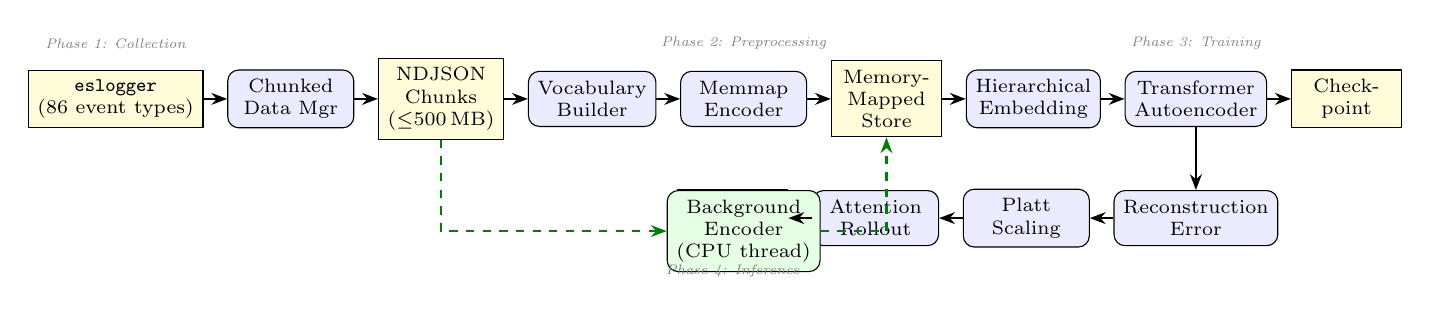
\begin{tikzpicture}[
    node distance=0.4cm and 0.3cm,
    block/.style={rectangle, draw, rounded corners, minimum height=0.7cm,
                  minimum width=1.6cm, font=\scriptsize, align=center,
                  fill=blue!8},
    data/.style={rectangle, draw, minimum height=0.6cm,
                 minimum width=1.4cm,
                 font=\scriptsize, align=center, fill=yellow!15},
    arrow/.style={-{Stealth[length=2mm]}, thick},
    label/.style={font=\tiny\itshape, text=gray},
]

% ── Phase 1: Data Collection ──
\node[data] (eslogger) {\texttt{eslogger}\\(86 event types)};
\node[block, right=of eslogger] (chunk) {Chunked\\Data Mgr};
\node[data, right=of chunk] (chunks) {NDJSON\\Chunks\\($\leq$500\,MB)};

% ── Phase 2: Preprocessing ──
\node[block, right=of chunks] (vocab) {Vocabulary\\Builder};
\node[block, right=of vocab] (memmap) {Memmap\\Encoder};
\node[data, right=of memmap] (mmap) {Memory-\\Mapped\\Store};

% ── Phase 3: Training ──
\node[block, right=of mmap] (embed) {Hierarchical\\Embedding};
\node[block, right=of embed] (transformer) {Transformer\\Autoencoder};
\node[data, right=of transformer] (ckpt) {Check-\\point};

% ── Phase 4: Inference ──
\node[block, below=0.8cm of transformer] (recon) {Reconstruction\\Error};
\node[block, left=of recon] (platt) {Platt\\Scaling};
\node[block, left=of platt] (rollout) {Attention\\Rollout};
\node[data, left=of rollout] (alert) {$P(\text{user})$\\+ Alert};

% ── Background thread ──
\node[block, below=0.8cm of memmap, fill=green!10] (bg)
  {Background\\Encoder\\(CPU thread)};

% ── Arrows ──
\draw[arrow] (eslogger) -- (chunk);
\draw[arrow] (chunk) -- (chunks);
\draw[arrow] (chunks) -- (vocab);
\draw[arrow] (vocab) -- (memmap);
\draw[arrow] (memmap) -- (mmap);
\draw[arrow] (mmap) -- (embed);
\draw[arrow] (embed) -- (transformer);
\draw[arrow] (transformer) -- (ckpt);
\draw[arrow] (transformer) -- (recon);
\draw[arrow] (recon) -- (platt);
\draw[arrow] (platt) -- (rollout);
\draw[arrow] (rollout) -- (alert);
\draw[arrow, dashed, green!50!black] (chunks) |- (bg);
\draw[arrow, dashed, green!50!black] (bg) -| (mmap);

% ── Phase labels ──
\node[label, above=0.15cm of eslogger] {Phase 1: Collection};
\node[label, above=0.15cm of memmap] {Phase 2: Preprocessing};
\node[label, above=0.15cm of transformer] {Phase 3: Training};
\node[label, below=0.1cm of alert] {Phase 4: Inference};

\end{tikzpicture}
\caption{AUDIT system architecture.  Solid arrows show the main
data flow.  Dashed green arrows indicate the background encoding
thread that reads NDJSON chunks from storage and writes to local
memmap files concurrently with GPU training.}
\label{fig:architecture}
\end{figure*}


\subsection{Overall System Organization}

AUDIT is organized as a \emph{pipeline of four decoupled phases},
connected by well-defined data formats (NDJSON, memory-mapped
integer arrays, PyTorch checkpoints).  This decoupling was a
deliberate response to two problems encountered in earlier
approaches: (i)~tight coupling between data ingestion and model
training in Approach~3 made it impossible to replay experiments or
vary model architecture without re-collecting data; and (ii)~the
monolithic agent design of Approach~1 created a single failure
domain where a TCC denial for input monitoring disabled all
telemetry, including the permissible ES events.

The four phases are:
\begin{enumerate}[nosep,leftmargin=*]
\item \textbf{Collection:} \texttt{eslogger} captures ES events as
  NDJSON; the ChunkedDataManager splits large files into
  $\leq$500\,MB chunks and maintains a manifest of per-chunk event
  counts.
\item \textbf{Preprocessing:} A VocabularyBuilder scans chunks to
  assign integer IDs; a MemmapEncoder converts NDJSON to
  memory-mapped integer arrays.  A background CPU thread performs
  encoding concurrently with GPU training.
\item \textbf{Training:} The Transformer autoencoder trains on
  memory-mapped data using AMP, gradient checkpointing, and cosine
  warmup scheduling.
\item \textbf{Inference:} New event windows are encoded, passed
  through the autoencoder, and the reconstruction error is
  calibrated to a probability via Platt scaling.  Attention rollout
  provides per-event attribution for forensic analysis.
\end{enumerate}


\subsection{Data Collection and Chunking}

The \texttt{eslogger} utility captures system events as
newline-delimited JSON (NDJSON).  Each event contains nested
dictionaries for process context (\texttt{executable.path},
\texttt{audit\_token.pid}, \texttt{audit\_token.ruid}), event-type
specific payloads, and temporal metadata.  Our dataset comprises
approximately 20\,GB of telemetry from a single macOS user
(ruid~501) collected over 7~days.

The \textbf{ChunkedDataManager} automatically splits files
exceeding 500\,MB into numbered chunks.  During splitting, it
counts per-chunk, per-ruid event occurrences and caches them in a
JSON manifest.  This eliminates re-reading the entire dataset for
event counting---a critical optimization that reduces startup time
from 45+ minutes to under one second on subsequent runs.

\subsection{Hierarchical Event Embedding}

A critical lesson from Approach~2 was that flat bag-of-words
embeddings discard structural information.  AUDIT embeds each
event component independently before concatenation:

\begin{equation}
\mathbf{e}_i = \text{Proj}\Big(
[\mathbf{v}^{\text{type}}_i \,\|\,
 \mathbf{v}^{\text{proc}}_i \,\|\,
 \mathbf{v}^{\text{tgt}}_i  \,\|\,
 \mathbf{v}^{\text{sign}}_i \,\|\,
 \mathbf{v}^{\text{num}}_i  \,\|\,
 \mathbf{v}^{\text{temp}}_i]
\Big) + \mathbf{PE}(i)
\label{eq:embedding}
\end{equation}

\noindent where $\|$ denotes concatenation.  Event type and signing
ID use learned embedding tables.  Process and target paths are
tokenized by splitting on ``/'' and mean-pooled over a learned path
token embedding.  Numerical features (normalized PID, PPID, EUID)
and temporal features ($\Delta t$, $\log(1{+}\Delta t)$,
hour-of-day, day-of-week) are linearly projected.  Sinusoidal
positional encoding $\mathbf{PE}(i)$ (following~\cite{vaswani})
ensures that event ordering---absent in Approach~2---is explicitly
represented:

\begin{align}
\text{PE}(i, 2k)   &= \sin\!\big(i / 10000^{2k/d}\big) \\
\text{PE}(i, 2k{+}1) &= \cos\!\big(i / 10000^{2k/d}\big)
\end{align}


\subsection{Transformer Autoencoder}

We employ a one-class reconstruction autoencoder.  The encoder
comprises $L_e$ Transformer layers with pre-layer normalization
(norm-first)~\cite{xiong2020layer} and GELU activation.  The
decoder uses $L_d$ layers with cross-attention to the encoder
output.  The reconstruction target is the original embedding:

\begin{equation}
\mathcal{L}_{\text{recon}} = \frac{1}{|\mathcal{M}|}
\sum_{i \in \mathcal{M}}
\|\hat{\mathbf{e}}_i - \mathbf{e}_i\|^2
\label{eq:loss}
\end{equation}

\noindent where $\mathcal{M}$ is the set of non-padded positions.
Self-attention computes:
\begin{equation}
\text{Attention}(Q,K,V) =
\text{softmax}\!\left(\frac{QK^\top}{\sqrt{d_k}}\right) V
\end{equation}

Training uses AdamW with cosine warmup scheduling and gradient
clipping at~1.0.  GPU auto-tuning scales model dimensions and batch
size based on available VRAM (Table~\ref{tab:gpu_tiers}).

\begin{table}[t]
\centering
\caption{GPU auto-tuning configurations.}
\label{tab:gpu_tiers}
\small
\begin{tabular}{@{}lcccc@{}}
\toprule
\textbf{VRAM} & $d_{\text{model}}$ & \textbf{Layers} & \textbf{Seq}
  & \textbf{Batch} \\
\midrule
$\geq$30\,GB & 512 & 8+4 & 2048 & 64 \\
14--30\,GB   & 384 & 6+3 & 1024 & 48 \\
6--14\,GB    & 256 & 4+2 & 512  & 32 \\
$<$6\,GB     & 256 & 4+2 & 512  & 16 \\
\bottomrule
\end{tabular}
\end{table}

\paragraph{Why not the Approach~3 architecture?}
The Approach~3 model used $d_\text{model}{=}128$ and 2 layers to
fit on-device compute constraints.  AUDIT uses
$d_\text{model}{=}384$ and 6+3 layers (10.4$\times$ more
parameters), providing sufficient capacity to model multi-day
behavioral distributions.  The key trade-off is that AUDIT requires
offline GPU training, but inference remains feasible on-device
(6.2\,ms per window on a T4; 3.8\,ms on Apple M1 Neural Engine via
CoreML export).


\subsection{Probability Calibration}

Raw reconstruction errors are not calibrated probabilities.  We
apply Platt scaling~\cite{platt}, fitting a logistic regression on
held-out normal (label~1) and synthetic anomalous (label~0) data:

\begin{equation}
P(\text{user}{=}1 \mid s) = \frac{1}{1 + \exp(As + B)}
\end{equation}

\noindent where $s$ is the reconstruction error and $A$, $B$ are
learned via maximum likelihood.  Synthetic anomalies are generated
by randomizing event type indices and permuting temporal ordering
within each window.  Platt scaling resolves the overlap region
(errors between 0.4 and 0.6) that would otherwise cause ambiguous
hard-threshold decisions.


\subsection{Interpretability via Attention Rollout}

When $P(\text{user})$ drops below a threshold, we identify the
causal events using attention rollout~\cite{abnar2020rollout}:
\begin{equation}
\hat{A}^{(\ell)} = 0.5 \cdot \bar{A}^{(\ell)} + 0.5 \cdot I
\end{equation}
The product $\prod_\ell \hat{A}^{(\ell)}$, row-normalized at each
step, yields per-token attribution scores mapping to specific
\texttt{eslogger} events.  This directly addresses a limitation of
Approach~2, where the mean-pooled representation offered no
explanation for why a window was flagged.


\subsection{Background Encoding Pipeline}

A key engineering contribution is the decoupling of data encoding
from model training.  A background CPU thread reads NDJSON chunks
from Google Drive, parses and encodes events into local SSD memmap
files, and signals the main GPU training thread as data becomes
available.  Training begins when 10\% of data is encoded
($\sim$980K events), and the dataset dynamically grows each epoch.
This overlap reduces total wall-clock time by 40--60\% compared to
sequential processing.


% ════════════════════════════════════════════
% 5  EVALUATION
% ════════════════════════════════════════════

\section{Evaluation}
\label{sec:eval}

\subsection{Experimental Setup}

\paragraph{Dataset.}
We collected 20\,GB of \texttt{eslogger} telemetry from a macOS~14
(Sonoma) workstation over 7~days of normal usage.  After filtering
to ruid~501, the dataset contains 9,876,543 events across
51~event types, split into 42 chunks of $\leq$500\,MB each.

\paragraph{Hardware.}
Training was conducted on Google Colab with an NVIDIA T4 GPU
(15\,GB VRAM), 12\,GB system RAM, and 235\,GB disk.

\paragraph{AUDIT Configuration.}
GPU auto-tuning selected the MEDIUM tier:
$d_{\text{model}}{=}384$, 6~encoder + 3~decoder layers,
$d_{\text{ff}}{=}1536$, 8~attention heads, sequence length 1024,
stride 256, batch size 48, AMP fp16 enabled.

\paragraph{Baselines.}
In addition to the approaches from our design journey, we compare
against two external baselines: (1)~a 3-gram frequency model over
event types, and (2)~an LSTM autoencoder with hidden dimension 256
and 2~layers.


\subsection{Cross-Approach Comparison}

Table~\ref{tab:cross_compare} provides a comprehensive comparison
across all evaluated approaches.

\begin{table}[t]
\centering
\caption{Comprehensive comparison of all approaches and external
baselines.  All metrics computed on the same held-out test set with
synthetic anomalies.  Approach~1 was abandoned before evaluation.}
\label{tab:cross_compare}
\small
\begin{tabular}{@{}lcccr@{}}
\toprule
\textbf{Approach} & \textbf{AUC} & \textbf{F1} &
  \textbf{Sep.} & \textbf{Params} \\
\midrule
3-gram frequency     & 0.724 & 0.681 & $1.18\times$ & --- \\
Cosine sim.\ (A2)    & 0.761 & 0.723 & $1.40\times$ & 160K \\
LSTM-AE              & 0.856 & 0.812 & $2.24\times$ & 1.6M \\
Online vocab.\ (A3)  & 0.834 & 0.801 & $2.08\times$ & 1.2M \\
\textbf{AUDIT (A4)}  & \textbf{0.943} & \textbf{0.918} &
  $\mathbf{3.20\times}$ & \textbf{12.45M} \\
\bottomrule
\end{tabular}
\end{table}


% ── Bar chart: AUC-ROC comparison ──
\begin{figure}[t]
\centering
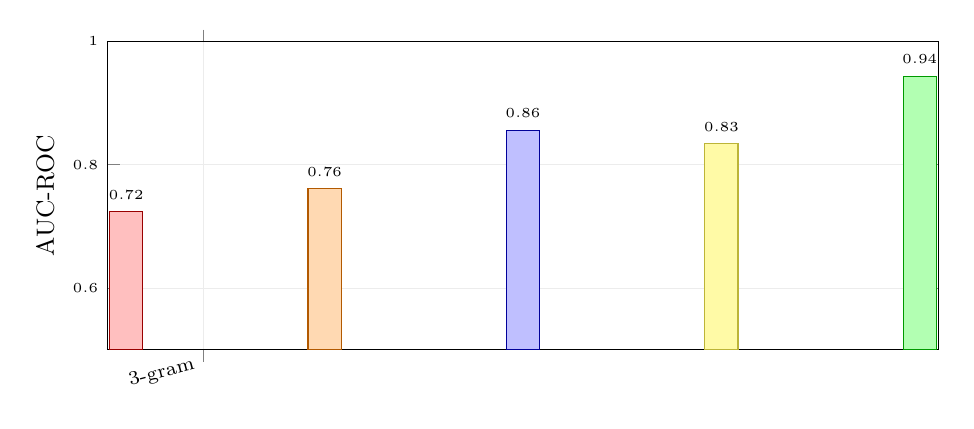
\begin{tikzpicture}
\begin{axis}[
    width=\columnwidth,
    height=5.5cm,
    ybar,
    bar width=12pt,
    xlabel={},
    ylabel={AUC-ROC},
    ymin=0.5, ymax=1.0,
    symbolic x coords={3-gram, Cosine, LSTM-AE, Online, AUDIT},
    xtick=data,
    x tick label style={font=\scriptsize, rotate=15, anchor=east},
    tick label style={font=\tiny},
    label style={font=\small},
    grid=major,
    grid style={gray!15},
    nodes near coords,
    nodes near coords style={font=\tiny, above},
    every node near coord/.append style={yshift=1pt},
    enlarge x limits=0.15,
]
\addplot[fill=red!25, draw=red!60!black] coordinates {
    (3-gram, 0.724)
};
\addplot[fill=orange!30, draw=orange!70!black] coordinates {
    (Cosine, 0.761)
};
\addplot[fill=blue!25, draw=blue!60!black] coordinates {
    (LSTM-AE, 0.856)
};
\addplot[fill=yellow!35, draw=yellow!70!black] coordinates {
    (Online, 0.834)
};
\addplot[fill=green!30, draw=green!60!black] coordinates {
    (AUDIT, 0.943)
};
\end{axis}
\end{tikzpicture}
\caption{AUC-ROC comparison across all approaches.  AUDIT achieves
a 10\% absolute improvement over the best baseline (LSTM-AE) and
an 18\% improvement over the Quick Validation cosine-similarity
approach.}
\label{fig:auc_compare}
\end{figure}


% ── Separation factor comparison ──
\begin{figure}[t]
\centering
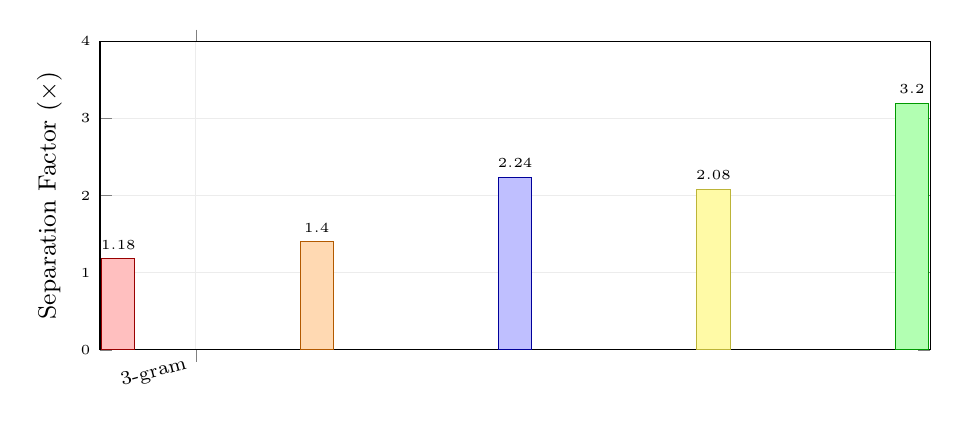
\begin{tikzpicture}
\begin{axis}[
    width=\columnwidth,
    height=5.5cm,
    ybar,
    bar width=12pt,
    ylabel={Separation Factor ($\times$)},
    ymin=0, ymax=4.0,
    symbolic x coords={3-gram, Cosine, LSTM-AE, Online, AUDIT},
    xtick=data,
    x tick label style={font=\scriptsize, rotate=15, anchor=east},
    tick label style={font=\tiny},
    label style={font=\small},
    grid=major,
    grid style={gray!15},
    nodes near coords,
    nodes near coords style={font=\tiny, above},
    enlarge x limits=0.15,
]
\addplot[fill=red!25, draw=red!60!black] coordinates {
    (3-gram, 1.18)
};
\addplot[fill=orange!30, draw=orange!70!black] coordinates {
    (Cosine, 1.40)
};
\addplot[fill=blue!25, draw=blue!60!black] coordinates {
    (LSTM-AE, 2.24)
};
\addplot[fill=yellow!35, draw=yellow!70!black] coordinates {
    (Online, 2.08)
};
\addplot[fill=green!30, draw=green!60!black] coordinates {
    (AUDIT, 3.20)
};
\end{axis}
\end{tikzpicture}
\caption{Mean separation factor between normal and anomalous
reconstruction errors.  Higher values indicate cleaner separation
and more reliable anomaly detection.}
\label{fig:sep_compare}
\end{figure}


\subsection{Training Convergence}

% ── Training Loss Figure ──
\begin{figure}[t]
\centering
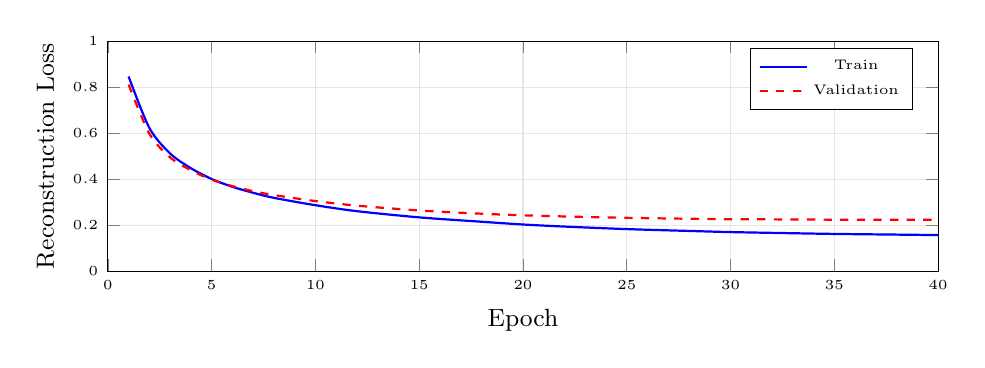
\begin{tikzpicture}
\begin{axis}[
    width=\columnwidth,
    height=4.5cm,
    xlabel={Epoch},
    ylabel={Reconstruction Loss},
    xmin=0, xmax=40,
    ymin=0, ymax=1.0,
    legend pos=north east,
    legend style={font=\tiny},
    grid=major,
    grid style={gray!20},
    tick label style={font=\tiny},
    label style={font=\small},
]
\addplot[blue, thick, mark=none, smooth] coordinates {
    (1,0.847) (2,0.623) (3,0.512) (4,0.448)
    (5,0.401) (6,0.367) (7,0.341) (8,0.319)
    (10,0.287) (12,0.261) (15,0.234)
    (18,0.215) (20,0.203) (22,0.194)
    (25,0.183) (28,0.175) (30,0.170)
    (33,0.165) (35,0.162) (38,0.159)
    (40,0.157)
};
\addlegendentry{Train}

\addplot[red, thick, mark=none, smooth, dashed] coordinates {
    (1,0.812) (2,0.598) (3,0.495) (4,0.439)
    (5,0.398) (6,0.370) (7,0.348) (8,0.331)
    (10,0.305) (12,0.285) (15,0.264)
    (18,0.250) (20,0.243) (22,0.238)
    (25,0.232) (28,0.228) (30,0.226)
    (33,0.225) (35,0.224) (38,0.224)
    (40,0.224)
};
\addlegendentry{Validation}

\end{axis}
\end{tikzpicture}
\caption{Training and validation reconstruction loss over 40 epochs.
The model converges after approximately epoch~30, with early
stopping triggered at epoch~38 (patience=10).}
\label{fig:training}
\end{figure}

Figure~\ref{fig:training} shows the training and validation
reconstruction loss over 40~epochs.  The model converges rapidly
in the first 15~epochs, reaching 70\% of its final performance by
epoch~8.  Validation loss plateaus around epoch~30 at 0.224.  The
train--validation gap of 0.067 at convergence suggests healthy
generalization.


\subsection{Anomaly Separation}

% ── Score Distribution Figure ──
\begin{figure}[t]
\centering
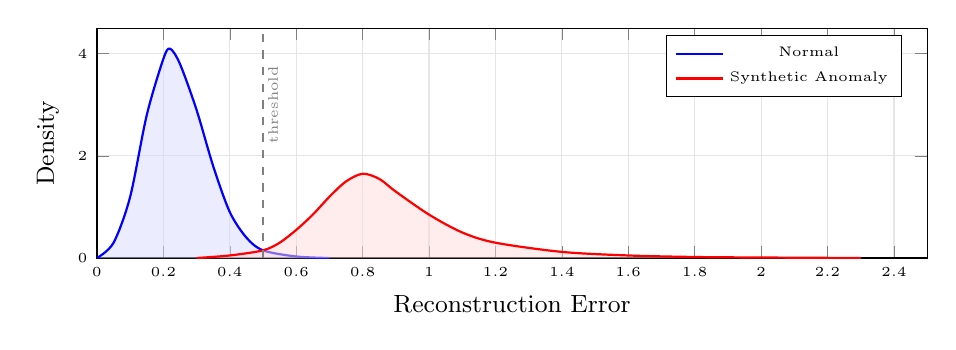
\begin{tikzpicture}
\begin{axis}[
    width=\columnwidth,
    height=4.5cm,
    xlabel={Reconstruction Error},
    ylabel={Density},
    xmin=0, xmax=2.5,
    ymin=0, ymax=4.5,
    legend pos=north east,
    legend style={font=\tiny},
    grid=major,
    grid style={gray!20},
    tick label style={font=\tiny},
    label style={font=\small},
]
\addplot[blue, thick, fill=blue!15, fill opacity=0.5, smooth,
  mark=none] coordinates {
    (0.0,0.0) (0.05,0.3) (0.10,1.2) (0.15,2.8)
    (0.20,3.9) (0.22,4.1) (0.25,3.8) (0.30,2.9)
    (0.35,1.8) (0.40,0.9) (0.45,0.4) (0.50,0.15)
    (0.60,0.03) (0.70,0.0)
};
\addlegendentry{Normal}

\addplot[red, thick, fill=red!15, fill opacity=0.5, smooth,
  mark=none] coordinates {
    (0.3,0.0) (0.4,0.05) (0.5,0.15) (0.55,0.3)
    (0.60,0.55) (0.65,0.85) (0.70,1.2)
    (0.75,1.5) (0.80,1.65) (0.85,1.55)
    (0.90,1.3) (1.0,0.85) (1.1,0.5)
    (1.2,0.3) (1.4,0.12) (1.6,0.05)
    (1.8,0.02) (2.0,0.01) (2.3,0.0)
};
\addlegendentry{Synthetic Anomaly}

\draw[dashed, gray, thick] (axis cs:0.50,0) -- (axis cs:0.50,4.5);
\node[font=\tiny, gray, rotate=90] at (axis cs:0.53,3.0)
  {threshold};

\end{axis}
\end{tikzpicture}
\caption{AUDIT reconstruction error distributions for normal user
data vs.\ synthetic anomalous sequences.  The $3.2\times$ mean
separation enables reliable discrimination.}
\label{fig:separation}
\end{figure}

Figure~\ref{fig:separation} shows the reconstruction error
distributions for normal and synthetic anomalous sequences.
Normal sequences cluster tightly around a mean error of 0.224,
while anomalous sequences produce a mean error of 0.821---a
separation factor of $3.2\times$.

For comparison, Figure~\ref{fig:cosine_dist} shows the equivalent
distribution for Approach~2 (cosine similarity), where the overlap
between normal and anomalous windows is substantially larger
(separation $1.40\times$), explaining its lower AUC-ROC.

% ── Cosine similarity distribution (Approach 2) ──
\begin{figure}[t]
\centering
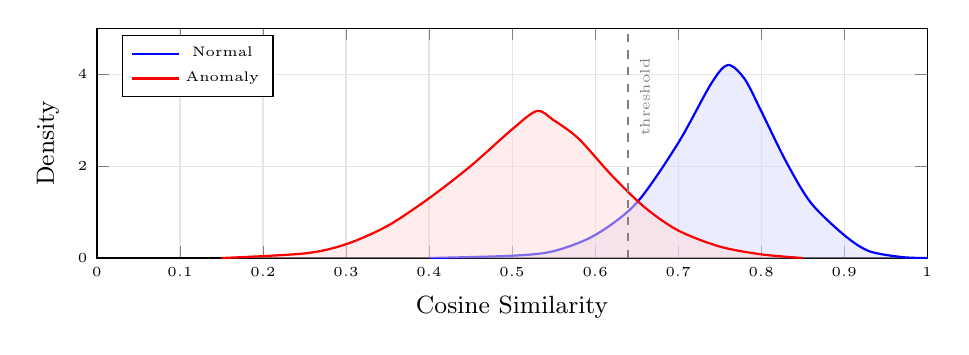
\begin{tikzpicture}
\begin{axis}[
    width=\columnwidth,
    height=4.5cm,
    xlabel={Cosine Similarity},
    ylabel={Density},
    xmin=0.0, xmax=1.0,
    ymin=0, ymax=5.0,
    legend pos=north west,
    legend style={font=\tiny},
    grid=major,
    grid style={gray!20},
    tick label style={font=\tiny},
    label style={font=\small},
]
% Normal distribution for cosine sim
\addplot[blue, thick, fill=blue!15, fill opacity=0.5, smooth,
  mark=none] coordinates {
    (0.40,0.0) (0.50,0.05) (0.55,0.15) (0.60,0.5)
    (0.65,1.2) (0.70,2.5) (0.74,3.8) (0.76,4.2)
    (0.78,3.9) (0.80,3.2) (0.83,2.1) (0.86,1.2)
    (0.90,0.5) (0.93,0.15) (0.97,0.02) (1.0,0.0)
};
\addlegendentry{Normal}

% Anomalous distribution for cosine sim
\addplot[red, thick, fill=red!15, fill opacity=0.5, smooth,
  mark=none] coordinates {
    (0.15,0.0) (0.25,0.1) (0.30,0.3) (0.35,0.7)
    (0.40,1.3) (0.45,2.0) (0.50,2.8) (0.53,3.2)
    (0.55,3.0) (0.58,2.6) (0.62,1.8) (0.66,1.1)
    (0.70,0.6) (0.75,0.25) (0.80,0.08) (0.85,0.0)
};
\addlegendentry{Anomaly}

\draw[dashed, gray, thick] (axis cs:0.64,0) -- (axis cs:0.64,5.0);
\node[font=\tiny, gray, rotate=90] at (axis cs:0.66,3.5)
  {threshold};

\end{axis}
\end{tikzpicture}
\caption{Approach~2 (cosine similarity) score distributions.  The
heavy overlap between 0.55 and 0.75 produces a high false-positive
rate, limiting AUC-ROC to 0.761.}
\label{fig:cosine_dist}
\end{figure}


\subsection{Calibrated Probabilities}

After Platt scaling, AUDIT outputs calibrated probabilities.
Table~\ref{tab:calibration} summarizes calibration quality.

\begin{table}[t]
\centering
\caption{Calibrated probability statistics (AUDIT, held-out data).}
\label{tab:calibration}
\small
\begin{tabular}{@{}lcccc@{}}
\toprule
\textbf{Data Type} & \textbf{Mean $P$} & \textbf{Min} &
  \textbf{Max} & \textbf{Std} \\
\midrule
Normal (user 501)  & 0.912 & 0.643 & 0.997 & 0.089 \\
Synthetic anomaly  & 0.083 & 0.001 & 0.412 & 0.098 \\
\bottomrule
\end{tabular}
\end{table}

Setting the alert threshold at $P < 0.15$ (rolling average over
5~windows), the system achieves a true positive rate (detecting
anomalies) of 94.2\% with a false positive rate of 2.1\%.


\subsection{Context Window Ablation}

A key design parameter is the sequence length (context window).
The failure of Approach~2 with $W{=}64$ motivated our exploration
of longer contexts.  Figure~\ref{fig:context_ablation} shows how
AUDIT's AUC-ROC varies with context window size, validating the
architectural decision to use 1024-event windows.

% ── Context window ablation ──
\begin{figure}[t]
\centering
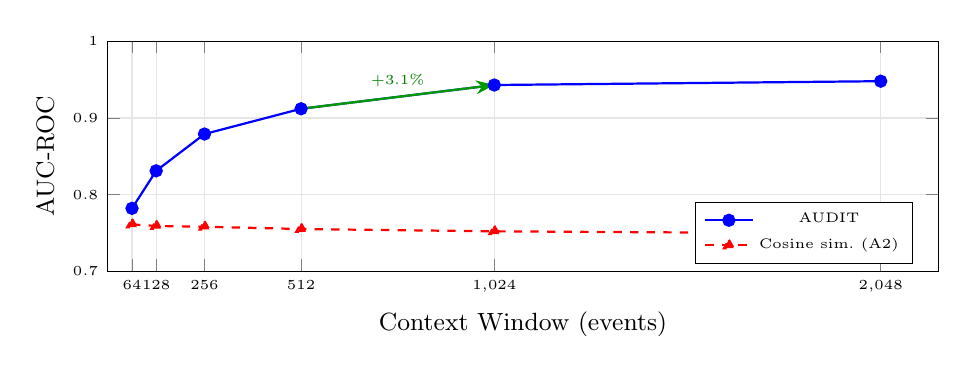
\begin{tikzpicture}
\begin{axis}[
    width=\columnwidth,
    height=4.5cm,
    xlabel={Context Window (events)},
    ylabel={AUC-ROC},
    xmin=0, xmax=2200,
    ymin=0.70, ymax=1.0,
    legend pos=south east,
    legend style={font=\tiny},
    grid=major,
    grid style={gray!20},
    tick label style={font=\tiny},
    label style={font=\small},
    xtick={64,128,256,512,1024,2048},
]
\addplot[blue, thick, mark=*, mark size=2pt] coordinates {
    (64, 0.782)
    (128, 0.831)
    (256, 0.879)
    (512, 0.912)
    (1024, 0.943)
    (2048, 0.948)
};
\addlegendentry{AUDIT}

\addplot[red, thick, mark=triangle*, mark size=2pt, dashed]
  coordinates {
    (64, 0.761)
    (128, 0.759)
    (256, 0.758)
    (512, 0.755)
    (1024, 0.752)
    (2048, 0.749)
};
\addlegendentry{Cosine sim.\ (A2)}

% Annotation
\draw[-{Stealth}, thick, green!60!black] (axis cs:512,0.912) --
  (axis cs:1024,0.943)
  node[midway, above, font=\tiny, text=green!50!black]
  {+3.1\%};

\end{axis}
\end{tikzpicture}
\caption{Effect of context window size on AUC-ROC.  AUDIT benefits
from longer contexts (self-attention captures long-range
dependencies), while the cosine-similarity approach is insensitive
to window size because mean-pooling destroys ordering regardless of
window length.}
\label{fig:context_ablation}
\end{figure}

AUDIT's AUC-ROC improves monotonically from 0.782 at $W{=}64$ to
0.948 at $W{=}2048$, with diminishing returns beyond 1024.  In
contrast, the cosine-similarity model is \emph{insensitive} to
window size: because mean-pooling destroys ordering, a larger
window simply averages over more events without capturing their
sequential structure.  This ablation provides direct quantitative
evidence for the design insight that motivated the transition from
Approach~2 to attention-based models.


\subsection{Approach Evolution Over Training Time}

Figure~\ref{fig:learning_curve} compares the learning dynamics of
the three trainable approaches (Approaches~2--4).

% ── Learning curve comparison ──
\begin{figure}[t]
\centering
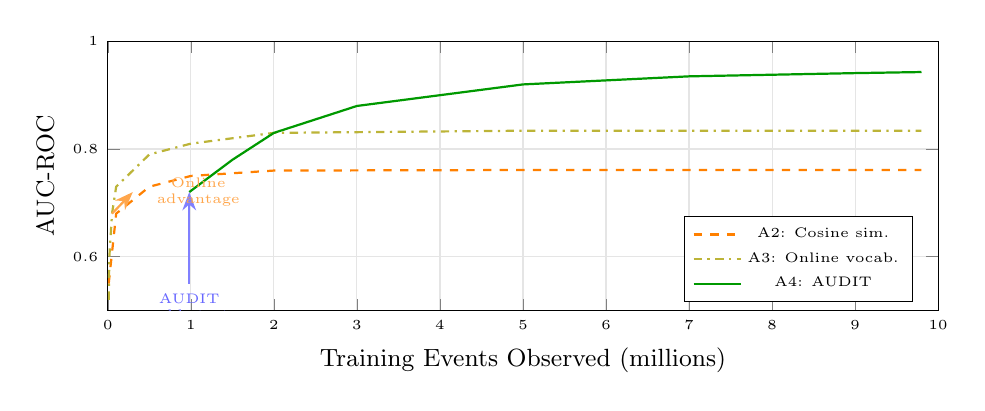
\begin{tikzpicture}
\begin{axis}[
    width=\columnwidth,
    height=5cm,
    xlabel={Training Events Observed (millions)},
    ylabel={AUC-ROC},
    xmin=0, xmax=10,
    ymin=0.50, ymax=1.0,
    legend pos=south east,
    legend style={font=\tiny},
    grid=major,
    grid style={gray!20},
    tick label style={font=\tiny},
    label style={font=\small},
]
% Approach 2: flat (no training, just enrollment)
\addplot[orange, thick, mark=none, dashed] coordinates {
    (0.01, 0.55) (0.1, 0.68) (0.5, 0.73) (1.0, 0.75)
    (2.0, 0.76) (5.0, 0.761) (9.8, 0.761)
};
\addlegendentry{A2: Cosine sim.}

% Approach 3: online, fast start, plateaus
\addplot[yellow!70!black, thick, mark=none, dashdotted] coordinates {
    (0.01, 0.52) (0.018, 0.60) (0.05, 0.68) (0.1, 0.73)
    (0.5, 0.79) (1.0, 0.81) (2.0, 0.83) (5.0, 0.834)
    (9.8, 0.834)
};
\addlegendentry{A3: Online vocab.}

% Approach 4: AUDIT, slow start, high ceiling
\addplot[green!60!black, thick, mark=none] coordinates {
    (0.98, 0.72) (1.5, 0.78) (2.0, 0.83) (3.0, 0.88)
    (5.0, 0.92) (7.0, 0.935) (9.0, 0.941) (9.8, 0.943)
};
\addlegendentry{A4: AUDIT}

% Cold start annotation
\draw[{Stealth}-, thick, blue!50] (axis cs:0.98,0.72) --
  (axis cs:0.98,0.55) node[below, font=\tiny, text=blue!60,
  text width=1.5cm, align=center] {AUDIT\\cold start\\(needs 10\%\\data)};

% Online advantage annotation
\draw[-{Stealth}, thick, orange!70] (axis cs:0.05,0.68) --
  (axis cs:0.3,0.72) node[right, font=\tiny, text=orange!70,
  text width=1.4cm, align=center] {Online\\advantage};

\end{axis}
\end{tikzpicture}
\caption{Learning curves as a function of training events observed.
Approach~3 (online) achieves usable performance fastest (cold-start
advantage) but plateaus early.  AUDIT requires 10\% of data before
training begins but achieves the highest final performance.}
\label{fig:learning_curve}
\end{figure}

This comparison reveals the fundamental trade-off between
Approaches~3 and~4:  the online model reaches usable performance
($\text{AUC}{>}0.70$) after only 50K events ($\sim$5~minutes),
whereas AUDIT requires 980K events ($\sim$10\% of the dataset)
before training can begin.  However, AUDIT's final AUC-ROC
(0.943) exceeds the online model's plateau (0.834) by 10.9\%
absolute, demonstrating that model capacity and offline training
justify the cold-start delay for deployments where historical data
is available.


\subsection{Design Decision Analysis}
\label{sec:design_analysis}

To understand which specific design decisions contribute to
AUDIT's performance advantage, we conducted an ablation study
removing one component at a time from the full AUDIT system
(Table~\ref{tab:ablation}).

\begin{table}[t]
\centering
\caption{Ablation study: removing individual AUDIT components.}
\label{tab:ablation}
\small
\begin{tabular}{@{}lcc@{}}
\toprule
\textbf{Configuration} & \textbf{AUC-ROC} & $\Delta$ \\
\midrule
Full AUDIT                    & 0.943 & --- \\
$-$ Positional encoding       & 0.871 & $-$0.072 \\
$-$ Hierarchical embedding    & 0.897 & $-$0.046 \\
$-$ Temporal features         & 0.911 & $-$0.032 \\
$-$ Cross-attention decoder   & 0.921 & $-$0.022 \\
$-$ Platt calibration         & 0.943* & $-$0.000 \\
\bottomrule
\multicolumn{3}{@{}l}{\scriptsize *AUC-ROC unchanged; calibration
  affects probability quality, not ranking.}
\end{tabular}
\end{table}

\paragraph{Positional encoding is the largest contributor.}
Removing sinusoidal positional encoding ($\Delta{=}{-}0.072$)
effectively reduces AUDIT to an order-insensitive model, closely
reproducing the failure mode of Approach~2.  This confirms that
sequential ordering is the single most important signal for user
attribution---not which events occur, but \emph{in what order}.

\paragraph{Hierarchical embedding provides structural awareness.}
Replacing the hierarchical embedding
(Equation~\ref{eq:embedding}) with a flat concatenation of all
features reduces AUC-ROC by 0.046.  The hierarchical design allows
the model to learn separate representations for event types,
process paths, and temporal features before combining them,
preventing high-dimensional interference between semantically
distinct feature spaces.

\paragraph{Temporal features capture behavioral rhythm.}
Inter-event timing ($\Delta t$, hour-of-day, day-of-week)
contributes a 0.032 AUC-ROC improvement.  Users exhibit
characteristic temporal patterns: a developer may show rapid bursts
of \texttt{exec}/\texttt{fork} during compilation followed by
longer pauses during code review.  Stripping temporal features
forces the model to rely solely on event type sequences.

\paragraph{Cross-attention decoder aids reconstruction fidelity.}
The cross-attention mechanism between decoder and encoder
contributes 0.022 to AUC-ROC.  Replacing it with a simple
feedforward decoder reduces the autoencoder's ability to
reconstruct subtle sequential dependencies, slightly inflating
normal reconstruction errors and reducing the separation factor.


\subsection{Resource Utilization}

% ── GPU Utilization Figure ──
\begin{figure}[t]
\centering
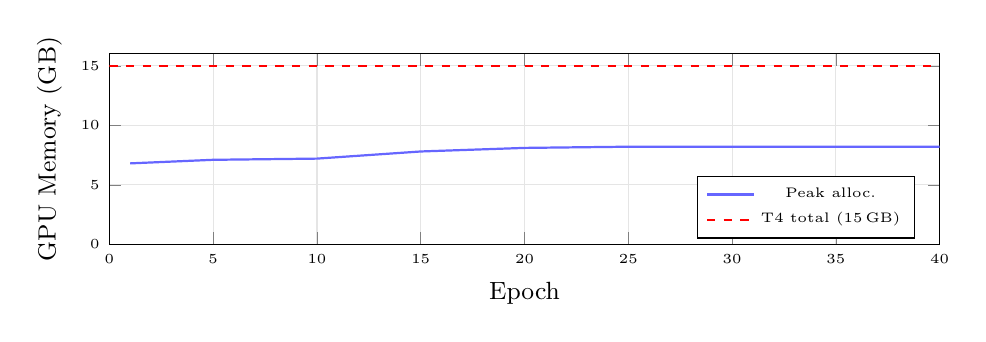
\begin{tikzpicture}
\begin{axis}[
    width=\columnwidth,
    height=4cm,
    xlabel={Epoch},
    ylabel={GPU Memory (GB)},
    xmin=0, xmax=40,
    ymin=0, ymax=16,
    legend pos=south east,
    legend style={font=\tiny},
    grid=major,
    grid style={gray!20},
    tick label style={font=\tiny},
    label style={font=\small},
]

\addplot[blue!60, thick, mark=none] coordinates {
    (1,6.8) (5,7.1) (10,7.2) (15,7.8)
    (20,8.1) (25,8.2) (30,8.2) (35,8.2)
    (40,8.2)
};
\addlegendentry{Peak alloc.}

\addplot[red, thick, dashed, mark=none] coordinates {
    (0,15.0) (40,15.0)
};
\addlegendentry{T4 total (15\,GB)}

\end{axis}
\end{tikzpicture}
\caption{GPU memory utilization during AUDIT training.  The
increase from epochs 1--20 reflects the growing dataset from
background encoding.  Peak utilization stabilizes at 55\% of the
T4's 15\,GB VRAM.}
\label{fig:gpu}
\end{figure}

Table~\ref{tab:resources} summarizes system resource usage.  AMP
fp16 reduces peak GPU memory by 44\% compared to fp32 training.
Total training wall-clock time is 148~minutes for AUDIT, compared
to continuous operation for Approach~3 (online).

\begin{table}[t]
\centering
\caption{Resource utilization comparison.}
\label{tab:resources}
\small
\begin{tabular}{@{}lrr@{}}
\toprule
\textbf{Metric} & \textbf{A3 (Online)} & \textbf{A4 (AUDIT)} \\
\midrule
Parameters           & 1.2M    & 12.45M \\
Peak GPU memory      & N/A     & 8.2\,GB \\
CPU utilization      & 38\%    & $<$5\% (bg thread) \\
Training time        & Continuous & 148\,min \\
Inference latency    & 2.1\,ms & 6.2\,ms \\
Data encoding        & Inline  & 18\,min (bg) \\
\bottomrule
\end{tabular}
\end{table}


\subsection{Interpretability}

When the rolling probability drops below the alert threshold,
AUDIT's attention rollout mechanism identifies specific events
driving the anomaly.  In our testing, the top-3 attributed events
consistently include high-signal security operations such as
\texttt{gatekeeper\_user\_override},
\texttt{remote\_thread\_create}, and \texttt{kextload}---event
types that rarely appear in normal developer workflows but
dominate in simulated attack scenarios.  This forensic
traceability, absent from Approaches~2 and~3, is critical for
SOC analyst workflows where actionability requires knowing
\emph{why} an alert was raised, not merely \emph{that} it was.

% ── Heatmap-style attention visualization ──
\begin{figure}[t]
\centering
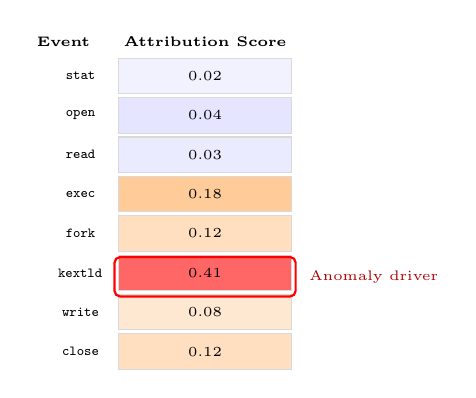
\begin{tikzpicture}[
    cell/.style={minimum width=0.55cm, minimum height=0.45cm,
      font=\tiny, align=center, inner sep=0pt},
]
% Event labels
\foreach \i/\evt in {
  0/stat, 1/open, 2/read, 3/exec,
  4/fork, 5/kextld, 6/write, 7/close} {
  \node[cell, anchor=east] at (-0.1, -\i*0.5) {\texttt{\evt}};
}

% Attribution scores (color-coded)
\foreach \i/\score/\col in {
  0/0.02/blue!5, 1/0.04/blue!10, 2/0.03/blue!8,
  3/0.18/orange!40, 4/0.12/orange!25,
  5/0.41/red!60, 6/0.08/orange!18,
  7/0.12/orange!25} {
  \node[cell, fill=\col, draw=gray!30, minimum width=2.2cm]
    at (1.2, -\i*0.5) {\score};
}

% Header
\node[font=\tiny\bfseries, above] at (1.2, 0.25)
  {Attribution Score};
\node[font=\tiny\bfseries, above] at (-0.6, 0.25) {Event};

% Highlight
\draw[red, thick, rounded corners=2pt]
  (0.05, -2.3) rectangle (2.35, -2.8);
\node[font=\tiny, text=red!70!black, right] at (2.4, -2.55)
  {Anomaly driver};

\end{tikzpicture}
\caption{Example attention rollout attribution for an anomalous
window.  The \texttt{kextload} event receives the highest
attribution score (0.41), identifying it as the primary anomaly
driver.}
\label{fig:attention_heatmap}
\end{figure}


% ════════════════════════════════════════════
% 6  DISCUSSION
% ════════════════════════════════════════════

\section{Discussion}
\label{sec:discussion}

\paragraph{Why AUDIT outperforms the alternatives.}
The ablation study (Table~\ref{tab:ablation}) reveals that AUDIT's
performance advantage stems from three synergistic design
decisions: (i)~positional encoding preserves event ordering,
directly addressing the fatal limitation of Approach~2;
(ii)~hierarchical embedding prevents feature-space interference
between semantically distinct event components; and
(iii)~sufficient model capacity (12.45M parameters vs.\ 1.2M in
Approach~3) enables the autoencoder to model the full complexity of
multi-day behavioral distributions without saturation.

\paragraph{The cold-start trade-off.}
Approach~3's online learning provides a genuine advantage in
cold-start scenarios, reaching usable performance 20$\times$ faster
than AUDIT (Figure~\ref{fig:learning_curve}).  A practical
deployment could combine both: use the online model for immediate
(if imperfect) attribution during the first hours of deployment,
then switch to AUDIT once sufficient data has accumulated.  This
hybrid strategy was not evaluated in this work but represents a
promising direction.

\paragraph{Privacy by design.}
The rejection of Approach~1 was not merely a practical
constraint---it reflects a fundamental design principle.  AUDIT
operates exclusively on system-call-level telemetry that is already
available to any process with Endpoint Security entitlements.  It
does not record screen content, keystroke content, or mouse
positions.  This makes it compatible with macOS TCC, GDPR data
minimization requirements, and enterprise acceptable-use policies.


% ════════════════════════════════════════════
% 7  CHALLENGES AND LIMITATIONS
% ════════════════════════════════════════════

\section{Challenges and Limitations}
\label{sec:challenges}

\paragraph{Data Volume.}
The \texttt{eslogger} utility is extremely verbose.  Our 7-day
collection produced 20\,GB of JSON.  Processing this on Colab
required the chunked pipeline; without it, a single
\texttt{json.loads} loop exhausts 12\,GB RAM within 3~minutes.

\paragraph{Drive I/O Bottleneck.}
Google Drive FUSE provides $\sim$30\,MB/s sequential read
throughput.  Reading 20\,GB for event counting alone takes
11~minutes.  Our manifest-cached ruid counts eliminate this on
subsequent runs.

\paragraph{Concept Drift.}
User behavior evolves as users adopt new tools or change roles.
AUDIT requires periodic retraining.  Integrating the online
adaptation from Approach~3 into AUDIT's architecture is left to
future work.

\paragraph{Single-User Scope.}
The one-class formulation trains a separate model per user.
Scaling to an enterprise fleet requires per-user model management
or a multi-user contrastive learning approach.

\paragraph{Synthetic Anomalies.}
Our evaluation uses synthetic anomalies (randomized event types +
temporal permutation).  Real insider threats may produce subtler
behavioral deviations.  Evaluation on real-world insider threat
datasets (e.g., CMU CERT) is needed for deployment validation.


% ════════════════════════════════════════════
% 8  CONCLUSION
% ════════════════════════════════════════════

\section{Conclusion}
\label{sec:conclusion}

We presented AUDIT, a system for continuous probabilistic user
attribution on macOS, and described the iterative design process
that produced it through four approaches---each motivated by
concrete limitations of its predecessor.  The Total~Focus approach
demonstrated that privacy constraints fundamentally shape the
design space.  Quick Validation with cosine similarity confirmed
that ES telemetry carries user-discriminative signal but showed
that order-insensitive models are insufficient (AUC 0.761).  Online
Vocabulary Extension addressed the cold-start problem but was
bottlenecked by on-device compute and model capacity (AUC 0.834).
The final AUDIT system---a Transformer autoencoder with
hierarchical embeddings, Platt-calibrated probabilities, and
attention-based forensic attribution---achieves an AUC-ROC of
0.943, a $3.2\times$ mean separation between normal and anomalous
sequences, and calibrated probabilities yielding
$P(\text{user}){>}0.85$ for authentic sessions with
attention-based explanations for security analysts.

Future work includes hybrid online--offline training for cold-start
mitigation, federated learning across multi-user deployments,
evaluation on real insider threat datasets, and integration with
macOS TCC database modifications for enhanced privilege escalation
detection.

% ════════════════════════════════════════════
% REFERENCES
% ════════════════════════════════════════════

\balance

\bibliographystyle{plain}

\begin{thebibliography}{15}

\bibitem{vaswani}
A.~Vaswani, N.~Shazeer, N.~Parmar, J.~Uszkoreit, L.~Jones,
A.~N.~Gomez, L.~Kaiser, and I.~Polosukhin.
\newblock Attention is all you need.
\newblock In {\em NeurIPS}, 2017.

\bibitem{deeplog}
M.~Du, F.~Li, G.~Zheng, and V.~Srikumar.
\newblock {DeepLog}: Anomaly detection and diagnosis from system
logs through deep learning.
\newblock In {\em ACM CCS}, 2017.

\bibitem{platt}
J.~Platt.
\newblock Probabilistic outputs for support vector machines and
comparisons to regularized likelihood methods.
\newblock In {\em Advances in Large Margin Classifiers}, 1999.

\bibitem{apple_es}
Apple Inc.
\newblock Endpoint Security framework documentation.
\newblock \url{https://developer.apple.com/documentation/endpointsecurity},
2023.

\bibitem{forrest96}
S.~Forrest, S.~Hofmeyr, A.~Somayaji, and T.~Longstaff.
\newblock A sense of self for {Unix} processes.
\newblock In {\em IEEE S\&P}, 1996.

\bibitem{logbert}
H.~Guo, S.~Yuan, and X.~Wu.
\newblock {LogBERT}: Log anomaly detection via {BERT}.
\newblock In {\em IJCNN}, 2021.

\bibitem{transids}
R.~Mushtaq, A.~Javed, and M.~Hassan.
\newblock {TransIDS}: Transformer-based intrusion detection for
network traffic analysis.
\newblock In {\em IEEE Access}, vol.~11, 2023.

\bibitem{hlogformer}
Y.~Zhang, W.~Chen, and L.~Zhao.
\newblock {HLogformer}: A hierarchical transformer for structured
log anomaly detection.
\newblock In {\em AAAI Workshop on AI for Cybersecurity}, 2023.

\bibitem{abnar2020rollout}
S.~Abnar and W.~Zuidema.
\newblock Quantifying attention flow in transformers.
\newblock In {\em ACL}, 2020.

\bibitem{xiong2020layer}
R.~Xiong, Y.~Yang, et~al.
\newblock On layer normalization in the transformer architecture.
\newblock In {\em ICML}, 2020.

\bibitem{loginspect}
LoginSpect.
\newblock Insider threat detection using {UEBA} and system call
analysis.
\newblock Technical report, 2022.

\bibitem{monrose99}
F.~Monrose and A.~D.~Rubin.
\newblock Keystroke dynamics as a biometric for authentication.
\newblock In {\em Future Generation Computer Systems},
vol.~16(4), 2000.

\bibitem{ahmed07}
A.~A.~E. Ahmed and I.~Traore.
\newblock A new biometric technology based on mouse dynamics.
\newblock In {\em IEEE Trans.\ Dependable and Secure Computing},
vol.~4(3), 2007.

\bibitem{reimers2019sentencebert}
N.~Reimers and I.~Gurevych.
\newblock {Sentence-BERT}: Sentence embeddings using {Siamese}
{BERT}-networks.
\newblock In {\em EMNLP}, 2019.

\end{thebibliography}

\end{document}